\documentclass[11pt,a4paper]{article}

%, Page Geometry & Layout ,
\usepackage[margin=1in]{geometry}
\usepackage[utf8]{inputenc}
\usepackage[T1]{fontenc}
\usepackage{lmodern}

%, Core Math & Symbols ,
\usepackage{amsmath,amssymb,amsfonts,amsthm}

%, Graphics, Tables & Formatting ,
\usepackage{graphicx}
\usepackage{booktabs}
\usepackage{microtype}
\setlength{\emergencystretch}{2em}
\usepackage{setspace}
\setstretch{1.12}

%, Tables ,
\usepackage{array}
\usepackage{multirow}
\usepackage{tabularx}
\renewcommand{\arraystretch}{1.15}
\setlength{\tabcolsep}{6pt}
\newcolumntype{R}{>{\raggedleft\arraybackslash}X}
\newcolumntype{L}{>{\raggedright\arraybackslash}X}
\newcommand{\tabfont}{\footnotesize}
\newcommand{\thead}[1]{\footnotesize\textbf{#1}}

%, Captions ,
\usepackage{caption}
\captionsetup{font=small, labelfont=bf}

%, Lists ,
\usepackage{enumitem}
\setlist[itemize]{leftmargin=1.5em,itemsep=2pt,topsep=4pt,parsep=0pt}
\setlist[enumerate]{leftmargin=1.8em,itemsep=2pt,topsep=4pt,parsep=0pt}

%, Colors ,
\usepackage[table,dvipsnames]{xcolor}
\definecolor{arblue}{HTML}{2A78D6}
\definecolor{dgorange}{HTML}{EB6834}
\definecolor{llaqua}{HTML}{1BAF7A}
\definecolor{linkc}{HTML}{1B3A5C}

%, Hyperlinks & Metadata ,
\usepackage[
    colorlinks=true,
    linkcolor=linkc,
    citecolor=linkc,
    urlcolor=linkc,
    pdfauthor={Aleksandr Kaigorodov},
    pdftitle={When Block-Diffusion Language Models Are Faster},
    pdfsubject={Block-structured decoding cost analysis},
    pdfkeywords={diffusion LLM, block decoding, latency, structured output}
]{hyperref}

%, Model shorthands ,
% NB: \ARthree renders AR-30B (the name is an AR-3B-era leftover).
\newcommand{\ARthree}{\textsc{ar-30b}}
\newcommand{\DG}{\textsc{dg}}
\newcommand{\LLaDA}{\textsc{llada-8b}}

%, Macros (numbers from results/) ,
% =============================================================================
%  macros.tex — every number the paper cites, in one place.
%
%  Rule: every measurement is a macro here, and the comment on its line names
%  the artifact it was read from. Section files may hardcode derived ratios
%  (e.g., 2.5×) and structural constants (e.g., 12 fields, $K{=}8$) for
%  readability, but raw measurements (latencies, F1 scores, energy) must be
%  macros. paper/verify_numbers.py checks provenance blocks and decimal-place
%  policy; the figure builder (paper/figures/make_figures.py) prints what it
%  plotted so the two can be diffed.
% =============================================================================

% --- Pinned stack -------------------------------------------------- (#57) --
\newcommand{\gpuModel}{NVIDIA A100 80GB PCIe}
% prompt_token_count in every DG cell (issue68_dg_L*.json, 42 files). The AR
% cells run shorter prompts (992); 1,077 is the DG figure the crossover is
% calibrated at. Was 1,047 -- a stale constant from docs/edr/005, no artifact.
\newcommand{\refPrompt}{1{,}077}

% --- Quality, 9-field vs 12-field ----- results/issue43_nine_field_f1.json --
\newcommand{\arThreeBFnine}{0.852}     % dense AR-3B (Qwen2.5-3B), L=256, 9-field, re-scored (#43)
\newcommand{\qualityGap}{0.000}        % |9-field difference|
\newcommand{\twelveGap}{0.041}         % 12-field difference, AR-favoured

% --- Cost laws ------------- results/anchors/*.json, results/issue68_*.json --
% AR-30B (arBase/arSlope/crossoverL): results/issue111_qwen3_serial_sweep.json
%   cost_law.{intercept_ms,slope_ms_per_token,crossover_L_star}.
%   Corrected serial-sweep artifact carries vLLM 0.25.1 provenance.
%   This fit uses cell means, not event medians; see v8 Section 2.
\newcommand{\arBase}{34.6}        % ms, AR-30B MoE serial intercept (Qwen3-30B-A3B)
\newcommand{\arSlope}{7.2}       % ms/token, AR-30B MoE serial decode slope
\newcommand{\dgBase}{378.8}       % ms, DG base at K=8
\newcommand{\dgStep}{119.5}       % ms, median of the 7 measured canvas steps
\newcommand{\dgStepLo}{113.1}     % ms, smallest measured step (1280->1536)
\newcommand{\dgStepHi}{122.6}     % ms, largest measured step (256->512)
\newcommand{\canvasLength}{256}   % tokens per canvas

% Anchors, five repeats each -------- results/anchors/anchor_remeasure.json --
% Per-event dispersion: n=2000 (issue #120, was n=300 where p99.9==max)
% results/anchors/dg_L256_r1_preds.jsonl, ar3b_L256_n2000_preds.jsonl
\newcommand{\arEventCV}{0.1}     % % CV over 2000 per-event latencies (AR-3B dense)
\newcommand{\dgEventCV}{16.9}
\newcommand{\arMaxMed}{1.03}      % max / median per-event latency (AR-3B dense)
\newcommand{\dgMaxMed}{3.07}

% --- Crossovers ------- derived from arBase/arSlope/dgBase above --------------
% NB: models/decision/procedure.py CONSTANTS updated to match (#113 0.5e).
\newcommand{\crossoverL}{48}       % tokens: (dgBase - arBase) / arSlope, serial mode
\newcommand{\crossoverLambda}{2.6} % ev/s: 1000 / dgBase (unchanged — DG base same)

% --- Input length, the second variable ------ results/issue44_*_sweep.json --
\newcommand{\inputSlopeRatio}{2.6} % dgInputSlope / arInputSlope (0.1/0.038)

% --- Base decomposition ------------------- results/issue44_dg_ksweep_K*.json --
\newcommand{\kfitBase}{296.1}      % ms, K-independent term (NOT interpretable as a floor; see #70)
\newcommand{\kfitSlope}{2.6}      % ms per denoising step
\newcommand{\kfitRsq}{0.49}
% Superseded: the fitted intercept (296.1) is not a measured floor. R^2=0.49
% and the curve saturates above K=16, so the linear term is a poor description.
% The 93.5%/6.5% split it produced over-attributes to the floor by ~5x.
% Replaced by two measurement-based bounds (issue #70):
% Floor share <=53% (from T(2)=201.7ms), denoising share >=32% (from canvas step 119.5ms).
% Values are hardcoded in Appendix 10 (appendix_decomp.tex).

% --- Batching ------------------- results/issue42_batching.json, appD, dInfer --
% NB: #42 was run on the dense AR-3B (Qwen2.5-3B-Instruct), NOT the AR-30B MoE.
% The AR-30B MoE multiplier is 24.7x (results/issue111_qwen3_batch_sweep.json).
\newcommand{\cacheOnMult}{42.8}    % dense AR-3B, prefix caching on   (#42)
\newcommand{\cacheOffMult}{26.8}   % dense AR-3B, prefix caching off  (#42)
\newcommand{\dgBatchVllmHi}{1.7}   % DG under vLLM, L=128 (lower bound)

% Energy values for v8 are bound to source artifacts below.

% --- Deployment pair ------ results/issue_evidence_ar1b_*.json, issue68_*.json --
\newcommand{\dgWeights}{52.0}          % GB, bf16

% --- Defect magnitudes ------------------------------ CHECKLIST.md, #65 -----
\newcommand{\defectOneFBefore}{0.779}
\newcommand{\defectOneFAfter}{0.844}
\newcommand{\defectTwoBefore}{1841.6}
\newcommand{\defectTwoAfter}{413.3}
\newcommand{\defectTwoRatio}{4.5}
\newcommand{\defectThreeBefore}{0.599}
\newcommand{\defectThreeAfter}{0.826}
\newcommand{\defectFourBefore}{0}
\newcommand{\defectFourAfter}{100}
\newcommand{\rambleRate}{96}      % % of AR outputs with >1 JSON object at L=512

% --- Truncation regime -------------------------- results/issue43/*.json -----
\newcommand{\arFOneTwentyEight}{0.669}   % AR-3B (dense) 9-field F1 at L=128
\newcommand{\dgFOneTwentyEight}{0.311}   % DG    9-field F1 at L=128
\newcommand{\arValidTwentyEight}{66.7}   % AR-3B (dense) schema-valid % at L=128
\newcommand{\dgValidTwentyEight}{1.0}    % DG schema-valid % at L=128

% --- Generalisation to HDFS ---------------------- results/issue67_*.json ----
\newcommand{\hdfsStep}{120.5}     % ms, DG canvas step on HDFS
\newcommand{\bglStep}{118.5}      % ms, DG canvas step on BGL (same cells)

% --- Canvas tuning -------------------------- results/issue66_canvas_*.json --
\newcommand{\canvasOneTwentyEightBase}{368.5}  % ms at canvas=128
\newcommand{\canvasOneTwentyEightFone}{0.864} % 9-field F1 at canvas=128

% --- K as a runtime quality knob --------- results/issue44_dg_ksweep_K*.json --
\newcommand{\kFourPninetynine}{394.3} % ms
\newcommand{\kFourFone}{0.790}
\newcommand{\kEightFone}{0.853}


% --- v8 audited primary-pair statistics and corrected energy ---
\newcommand{\arMedian}{924.4} % results/anchors/ar30b_stats.json ar30b_bgl.p50_ms
\newcommand{\arCiLo}{918.2} % results/anchors/ar30b_stats.json ar30b_bgl.p50_ci_95.0
\newcommand{\arCiHi}{926.5} % results/anchors/ar30b_stats.json ar30b_bgl.p50_ci_95.1
\newcommand{\arPninetyNine}{1400.4} % results/anchors/ar30b_stats.json ar30b_bgl.p99_ms
\newcommand{\arThirtyCV}{12.25} % results/anchors/ar30b_stats.json ar30b_bgl.cv_pct
\newcommand{\dgMedian}{379.7} % results/anchors/ar30b_stats.json dg_bgl.p50_ms
\newcommand{\dgCiLo}{379.1} % results/anchors/ar30b_stats.json dg_bgl.p50_ci_95.0
\newcommand{\dgCiHi}{380.4} % results/anchors/ar30b_stats.json dg_bgl.p50_ci_95.1
\newcommand{\dgPninetyNine}{490.7} % results/anchors/ar30b_stats.json dg_bgl.p99_ms
\newcommand{\dgThirtyCV}{16.92} % results/anchors/ar30b_stats.json dg_bgl.cv_pct
\newcommand{\hdfsMedian}{1082.3} % results/anchors/ar30b_stats.json ar30b_hdfs.p50_ms
\newcommand{\hdfsCiLo}{1077.9} % results/anchors/ar30b_stats.json ar30b_hdfs.p50_ci_95.0
\newcommand{\hdfsCiHi}{1106.0} % results/anchors/ar30b_stats.json ar30b_hdfs.p50_ci_95.1
\newcommand{\seedCV}{0.04} % results/anchors/ar30b_stats.json ar30b_bgl.seed_p50_cv_pct
\newcommand{\arEnergy}{166.5} % results/issue111_ar30b_energy.json energy_per_event_j
\newcommand{\dgEnergy}{4.2} % results/issue_energy_measurement.json measurements.1.idle_subtracted_energy_per_event_j
\newcommand{\arBatchMult}{24.7} % results/issue111_qwen3_batch_sweep.json multiplier


\graphicspath{{./}{figures/}}

\title{\textbf{When Block-Diffusion Language Models Are Faster:\\
Latency, Throughput, and Quality in Structured Log Extraction}}

\author{
  \textbf{Aleksandr Kaigorodov, Yandex}
}

\date{}

\begin{document}

\maketitle

\begin{abstract}
Online log processing needs usable records before a response deadline;
a correct answer arriving too late may miss its purpose. We compare
DiffusionGemma with the autoregressive Qwen3 model on structured extraction
from BlueGene/L (BGL) system logs, using saved serial runs on an
NVIDIA A100 graphics processing unit. Diffusion refines multiple token
positions in parallel, whereas standard autoregressive decoding emits tokens
sequentially. With one request at a time, median generation latency is
380 versus 924\,ms, a $2.4\times$ advantage for diffusion. Empirical cost
models explain how output length and block boundaries affect this comparison;
long natural outputs remain an extrapolation. The latency gap motivates
diffusion for deadline-bound extraction when its output meets the task's
quality and validity requirements. On 300 shared events, token-overlap extraction
scores are 0.870 for Qwen3 and 0.852 for diffusion; this is a latency--quality
tradeoff. Autoregressive throughput benefits more from batching
in the tested configurations. The practical choice therefore depends on
response time, acceptable quality, concurrency, and resource utilization.
\end{abstract}

\begin{center}
\captionsetup{hypcap=false}
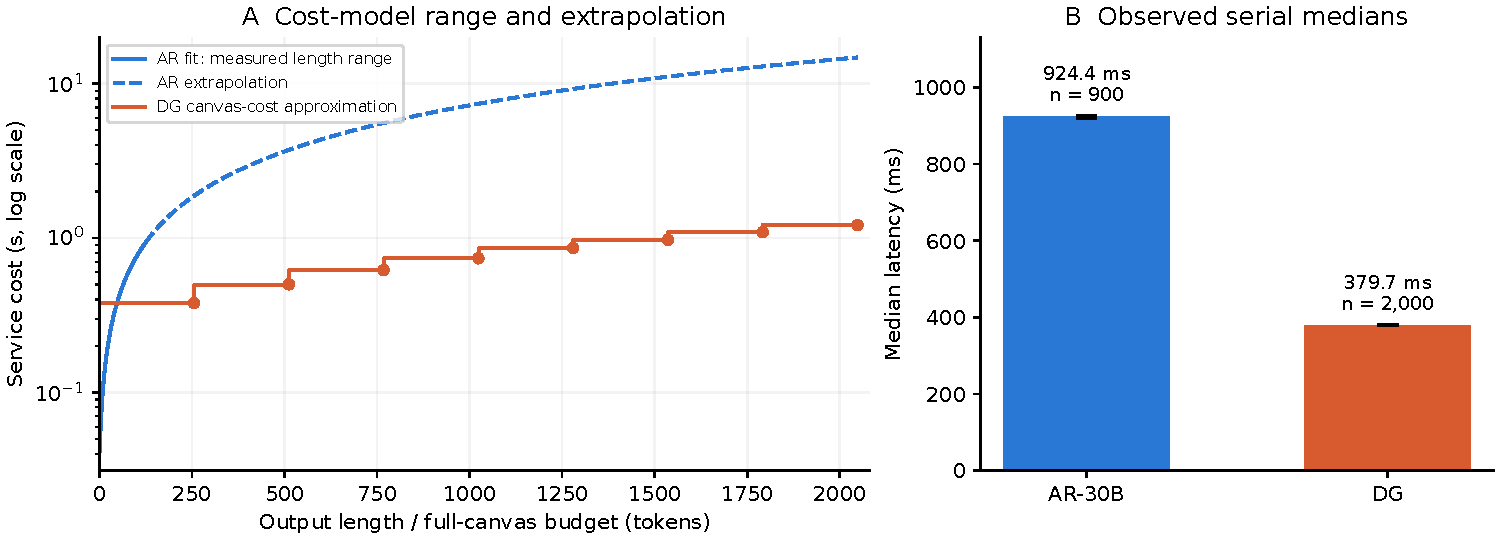
\includegraphics[width=\linewidth]{figures/fig1_v8.pdf}
\captionof{figure}{Speed and its scope. Left: autoregressive (AR) cost versus
output length and DiffusionGemma (DG) cost versus decoded block budget.
The dashed AR curve extrapolates beyond measured natural output lengths.
Right: measured serial medians with 95\% confidence intervals on BlueGene/L
logs (AR: 900 events; DG: 2,000). Longer-output task speedups are projections.}
\label{fig:shapes}
\end{center}
\clearpage

\section{Introduction}
\label{sec:intro}

An online log processor may need to identify an event and choose a follow-up
check before a response deadline. A correct answer arriving after that
deadline can still help later analysis, but cannot support the intended
timely decision. This makes response latency a different objective from
processing as many requests per second as possible. The operational goal
is to maximize the fraction of problems resolved correctly before their
deadline, while retaining the required quality standard.

Autoregressive (AR) decoding generates tokens, the model's units of text,
one after another. Block diffusion instead refines a fixed-size block of
token positions, called a \emph{canvas}, through several passes before
moving to the next block. It can therefore produce a structured response
with fewer sequential decoding steps. Figure~\ref{fig:shapes} connects this
intuition to the measured latency gap and conditional output-length model.

Our primary comparison is Qwen3-30B-A3B (AR-30B)~\cite{qwen3} versus
DiffusionGemma-26B-A4B (DG)~\cite{diffusiongemma}. These similarly sized mixture-of-experts
models activate only a subset of their parameters for each token:
AR has approximately 30 billion total and 3 billion active parameters,
while DG has 26 billion total and 4 billion active parameters.
They are comparable in scale, not identical in training or capability.
Experiments with dense Qwen2.5-3B (AR-3B) and the separate LLaDA-8B
diffusion model provide supporting evidence. Section~\ref{sec:survives}
uses one explicitly labeled AR-3B timing illustration; details of these
secondary experiments remain in Appendix~\ref{app:secondary}.

\noindent\begin{minipage}{\linewidth}
\paragraph{Three takeaways.}
\begin{enumerate}
\item \textbf{Diffusion returns sooner in the measured serial workload.}
The primary pair has median generation times of approximately 924\,ms
for AR and 380\,ms for DG, a $2.4\times$ ratio.
\item \textbf{The latency gap changes which responses fit a time budget.}
Within 500\,ms, 99.8\% of DG generations finish in the saved runs,
compared with none from this AR configuration.
\item \textbf{Quality and concurrency determine whether that speed is useful.}
On 300 shared events, nine-field F1 is 0.870 for AR and 0.852 for DG.
The scores are close, with a small DG deficit; AR also gains
more throughput from batching.
\end{enumerate}
\end{minipage}

\paragraph{Task and measures.}
Each BlueGene/L (BGL) system log line from Loghub~\cite{loghub} is converted to a JavaScript Object
Notation (JSON) record with twelve named fields. We evaluate nine fields:
seven structural fields and two anomaly fields. The other three describe
events, affected entities, and actions, whose semantic quality is not
independently labeled. Field-F1 measures token overlap with parser-derived
reference values; it is the harmonic mean of precision and recall, averaged
equally over scored fields. Schema validity checks required fields,
types, and allowed values. Neither guarantees a correct downstream decision.

We use saved serial runs on an NVIDIA A100 graphics processing unit (GPU)
with 80\,GB memory. Both models use vLLM serving software and greedy
decoding, without random sampling. DG uses eight refinement passes
($K=8$) and a 256-position canvas ($C=256$); AR has a 256-token maximum
output budget. The latency comparison pools three AR runs on
300 events and one DG run on 2,000 events. Paired quality uses the first
300 shared events, not the pooled timing samples.
Preparation, scoring, and conflicting DG software-version metadata
are documented in Appendix~\ref{app:protocol}.

\paragraph{Roadmap.}
We explain the cost models, compare the primary pair's quality and
generation-time budgets, then discuss batching and how latency savings
can accumulate across dependent actions. The appendices retain protocol details, smaller-model
studies, and exploratory results without mixing them into the main comparison.

\section{Why output length changes the comparison}
\label{sec:laws}

Standard AR decoding adds one token at a time, reusing its key-value (KV)
cache of earlier computation. DG refines positions together inside each
canvas and generates canvases sequentially. Its encoder caches input
context while its decoder refines the active canvas~\cite{diffusiongemma}.
Parallel output positions therefore do not mean all generation work
happens at once.

\begin{center}
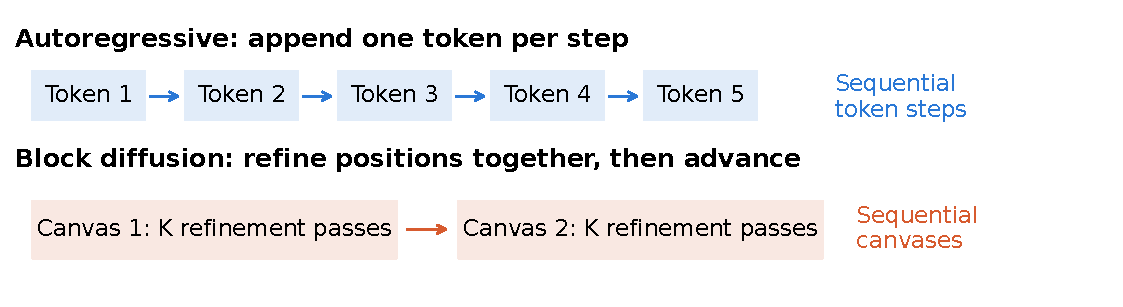
\includegraphics[width=.94\linewidth]{figures/decoding_schematic.pdf}
\captionof*{figure}{Decoding schedules (schematic). AR advances token by
token; DG refines each canvas over $K$ passes before starting the next.
These are execution patterns, not a timing scale.}
\end{center}

At a fixed prompt and decoding configuration, we estimate service time
$\widehat T$ in milliseconds by
\begin{align}
\label{eq:ar}
\widehat T_A(L) &= a_A+b_A L,\\
\label{eq:dg}
\widehat T_D(N_C) &= a_D+s_D(N_C-1),\qquad N_C\geq1.
\end{align}
Here $L$ is the generated token count and $N_C$ the number of decoded
canvases. The coefficients and units are listed below.

\begin{center}
\begin{tabular}{@{}llr@{}}
\toprule
Coefficient & Meaning & Fitted value \\
\midrule
$a_A$ & AR starting cost & \arBase\,ms \\
$b_A$ & AR incremental cost & \arSlope\,ms/token \\
$a_D$ & DG first-canvas cost & \dgBase\,ms \\
$s_D$ & DG additional-canvas cost & \dgStep\,ms \\
\bottomrule
\end{tabular}
\end{center}

Within the first canvas, the predicted times are equal at
\begin{equation}
\label{eq:lcross}
L^*=\frac{a_D-a_A}{b_A}
=\frac{\dgBase-\arBase}{\arSlope}\approx\crossoverL\quad\text{tokens}.
\end{equation}
The numerator is the difference in starting costs; dividing by AR's cost
per token gives the crossover length. Beyond this point, the model predicts
a diffusion advantage within the first canvas. Further canvases add cost,
so the comparison must be recalculated at each boundary.

This explains why longer required output can favor diffusion, but the
measured range matters. The AR fit covers only about 32--126 generated
tokens and uses mean times, whereas DG canvas costs summarize medians.
A fitted crossover is an approximate cost comparison, not proof of a
valid record or equal-quality speedup. Raising a maximum output budget
does not lengthen a response that has already reached its end-of-sequence
(EOS) stopping token. Appendix~\ref{app:secondary} gives a compact
budget-accounting example and supporting measurements.

\section{Primary-pair quality and latency}
\label{sec:wins}

\subsection{Quality on the same log events}
The relevant quality comparison is between AR-30B and DG themselves.
We re-score their saved outputs on the same 300 BGL events with the same
nine-field metric and parser-derived references. Table~\ref{tab:primaryquality}
places this comparison beside its generation times.

\begin{table}[ht]
\centering
\caption{Primary pair on 300 shared events. F1 measures extraction agreement;
schema validity checks record structure. These are paired-sample timings,
separate from the larger repeated latency sample.}
\label{tab:primaryquality}
\begin{tabular}{@{}lrr@{}}
\toprule
Measure & AR-30B & DG \\
\midrule
Nine-field F1 & 0.870 & 0.852 \\
Schema-valid records (\%) & 99.3 & 99.0 \\
Paired-sample median (ms) & 924.2 & 373.7 \\
\bottomrule
\end{tabular}

\end{table}

DG's extraction score is close to AR's, and a paired bootstrap analysis
supports a small average DG deficit. The saved outputs therefore show a
faster response with a modest loss on this metric, rather than equal
quality. Whether that tradeoff is acceptable depends on the task;
Appendix~\ref{app:protocol} reports the difference, uncertainty interval,
and scoring limits without choosing an equivalence margin after the fact.

\subsection{Reading a generation-time budget}
For the larger repeated timing sample, median latency is
\dgMedian\,ms for DG and \arMedian\,ms for AR-30B. The median describes
the middle request; a deadline asks a different question: what fraction
has finished by a specified time?

Figure~\ref{fig:distributions} answers that question directly. Pick a time
on the horizontal axis, move up to a model's curve, and read the percentage
of completed generations. At 1,000\,ms, nearly all DG responses have
finished, while about three quarters of AR responses have. A steep section
means many requests finish in a narrow time range.

\begin{figure}[ht!]
\centering
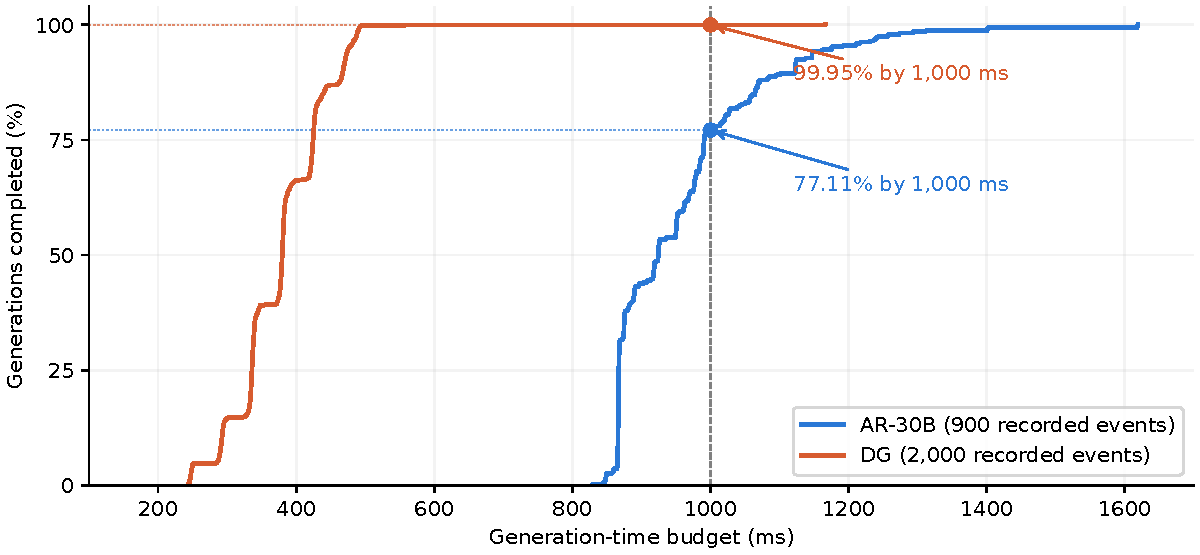
\includegraphics[width=.95\linewidth]{figures/fig12_v8.pdf}
\caption{Percentage of saved generations completed within each time budget
(AR-30B: 900 events across three runs; DG: 2,000 events).
Dots and guides show the 1,000\,ms example. These are generation times,
not end-to-end response times or correctness rates.}
\label{fig:distributions}
\end{figure}

\begin{table}[ht]
\centering
\caption{Generation-budget coverage (\%). Valid also requires the harness
schema check. All recorded events remain in the denominator; semantic
correctness and downstream processing are not assessed here.}
\label{tab:budgets}
\begin{tabular}{@{}rrrrr@{}}
\toprule
& \multicolumn{2}{c}{Completed} & \multicolumn{2}{c}{Valid and completed} \\
Budget (ms) & AR-30B & DG & AR-30B & DG \\
\midrule
500 & 0.00 & 99.80 & 0.00 & 98.50 \\
1000 & 77.11 & 99.95 & 76.44 & 98.65 \\
\bottomrule
\end{tabular}

\end{table}

At a 500\,ms generation budget, DG supplies structurally valid records
for most events and this AR configuration supplies none. This is a
concrete reason to evaluate DG for a time-constrained service, provided its
extraction quality meets the application's needs. It is not a claim that
every possible AR configuration misses the same target.

\section{Deployment constraints}
\label{sec:limits}

\paragraph{Batching and concurrency.}
AR-30B improves throughput by \arBatchMult$\times$ in its batching
experiment, whereas DG reaches up to $1.7\times$ in the tested
configurations. LLaDA-8B on the dInfer inference engine reaches approximately $1.2\times$.
The diffusion measurements are implementation-limited: the tested vLLM
path restricts mixed-phase batches, and dInfer was run without its
intended cache. They establish modest gains on those stacks, not an
upper bound on diffusion batching.

\begin{figure}[ht!]
\centering
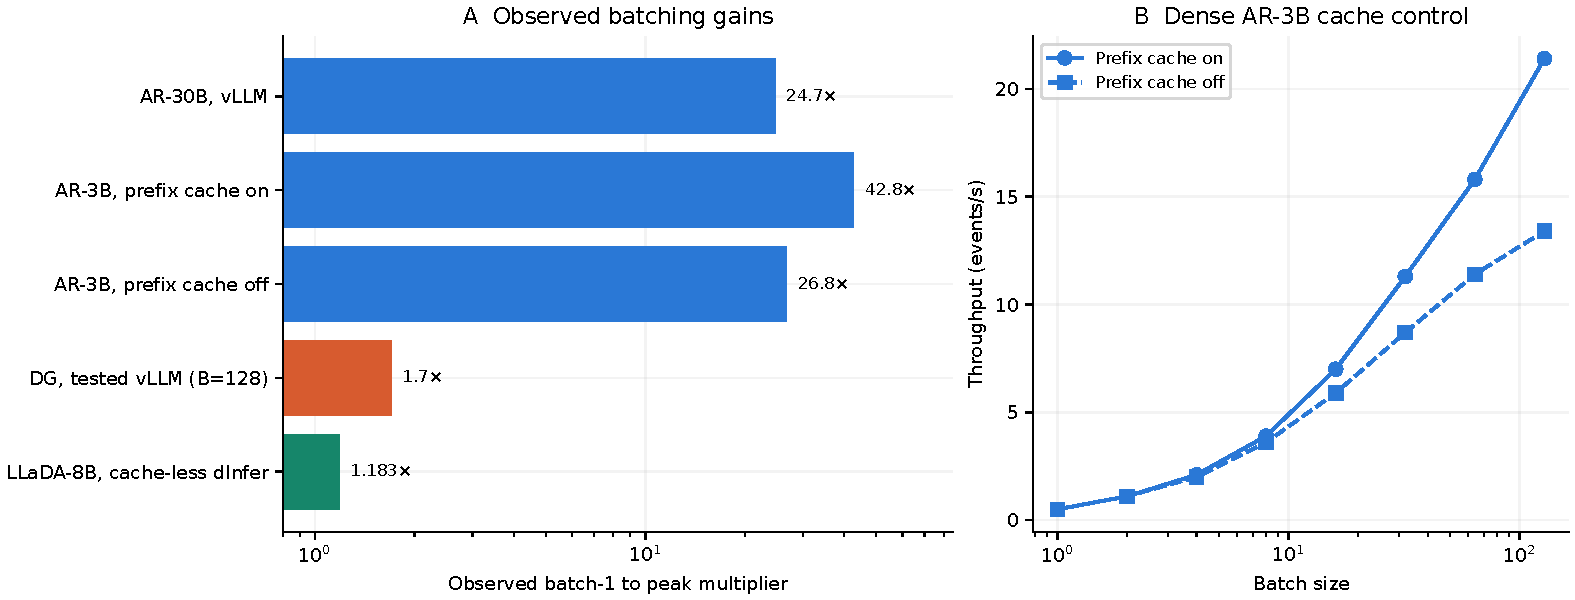
\includegraphics[width=\linewidth]{figures/fig6_batching.pdf}
\caption{Observed throughput multipliers for several model/runtime pairs.
The primary AR-30B result is approximately $25\times$. The cache-on/off
control uses dense AR-3B. Disabling cross-request
prefix caching lowers that model's multiplier from \cacheOnMult$\times$
to \cacheOffMult$\times$, so shared prefixes alone do not explain
its throughput gain. These controls do not identify a universal DG limit.}
\label{fig:batching}
\end{figure}

Sequential steps within one request chain cannot batch with each other,
but requests from independent chains can still overlap. Likewise,
interactivity and tenant isolation do not necessarily require a dedicated
batch-1 GPU. Deployment decisions should use measured arrival patterns,
scheduler behavior, and latency targets. Appendix~\ref{app:batching}
separates the cache observations from possible explanations.

\paragraph{Absolute and relative tails.}
In the repeated primary-pair measurements, AR-30B has CV
\arThirtyCV\% and max/median $1.75\times$, compared with
\dgThirtyCV\% and $3.07\times$ for DG. However, DG's absolute
p99 is \dgPninetyNine\,ms versus AR's \arPninetyNine\,ms.
A larger relative tail does not imply a slower absolute response or
a service-level agreement (SLA) violation. The relevant test is the specified latency percentile
under the intended arrival process. Sample maxima are not worst-case
bounds, and comparing maximum ratios across unequal sample sizes is
particularly fragile (Appendix~\ref{app:distributions}).

\paragraph{Prompt length and decoding settings.}
Longer prompts increase DG cost and can move the fitted crossover.
The input-slope comparison uses dense AR-3B and cannot be transferred
numerically to AR-30B. Canvas size and $K$ also change both cost and
quality. A joint sweep finds a better measured operating point than the
paper's reference setting: canvas 128, $K{=}8$ gives 368\,ms and
F1 0.864 versus 376\,ms and 0.853 at canvas 256, $K{=}8$.
These are point estimates on one sample, not a statistically established
improvement for all workloads (Appendix~\ref{app:input_canvas}).

\paragraph{Memory and co-residency.}
The nominal 52--60\,GB bf16 weight footprints of the primary pair
leave limited space for other large models on an 80\,GB GPU. Actual
capacity also depends on KV caches, activations, and runtime allocations.
A dense AR-1.5B has much smaller weights, but dividing GPU memory by
weight size cannot establish how many serving replicas fit or how their
throughput scales. We have not measured concurrent replicas, contention,
or isolation overhead, and make no linear co-residency speedup claim.

\paragraph{Cost accounting.}
At an assumed GPU rental rate $r$ dollars/hour, mean service time
$\bar t$ seconds/event, and busy fraction $u$, a simple single-instance
allocation is
\begin{equation}
 c_{\mathrm{event}}=\frac{r\bar t}{3600u}.
\end{equation}
This assumes the same GPU is rented throughout both busy and idle periods;
it excludes central processor, storage, networking, and retry costs. At fixed demand,
lower latency does not reduce the bill for an always-on GPU unless it
allows fewer provisioned resources or more useful work. A latency-based rental estimate therefore does not establish realized
annual savings. Batching economics should use measured throughput and
the quality requirement, rather than a serial latency ratio alone.

For a deadline-bound task, first establish which configurations return
acceptable records on time, then compare their costs. A configuration
that processes more records per second may still deliver each record too
late for that task. Conversely, the serial comparison does not show that
every AR configuration misses the target: scheduler, model, and decoding
choices require measurement at the intended load.

\section{Where faster serial responses can help}
\label{sec:survives}

\paragraph{Online extraction under a deadline.}
A log processor may need an event's severity and affected component before
deciding whether to request another check. Its response budget covers
queueing, generation, validation, and the decision. A correct record
received too late cannot support that timely action.

\begin{center}
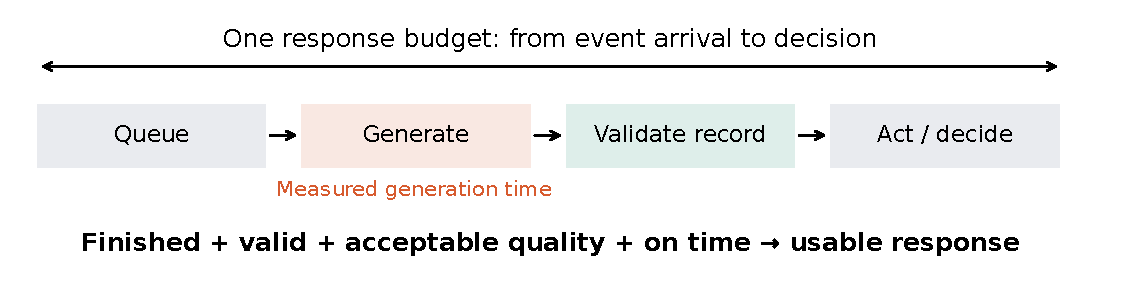
\includegraphics[width=.94\linewidth]{figures/deadline_path.pdf}
\captionof*{figure}{The full response path (schematic). Generation occupies
one stage; the remaining stages also consume the deadline.}
\end{center}

The completion fractions in \S\ref{sec:wins} quantify generation.
They make DG a useful candidate when this stage has a tight budget and
its quality is sufficient. A complete canvas still needs validation;
an on-time error does not become useful just because it arrived quickly.
End-to-end decisions require measurements of the remaining stages.

\paragraph{Dependent investigations and longer responses.}
In an investigation, the next query may depend on an earlier answer.
Such dependencies make per-call latency accumulate, even while other
investigations run concurrently. Lower latency can shorten the time to
the next useful observation. The saved chain experiment supports this
motivation using the smaller AR-3B baseline; it is reported separately
in Appendix~\ref{app:secondary}, not as an AR-30B chain benchmark.

A long response and a chain of responses are different workloads.
The first can spread DG's initial canvas cost over more required tokens;
the second repeats input processing and generation across dependent calls.
Both motivate evaluating diffusion, but neither guarantees a benefit at
arbitrary lengths. Long-form reasoning and repeated code generation also
require suitable quality. The exploratory code results in
Appendix~\ref{app:humaneval} show a substantial quality gap, so they do not
establish successful long investigations for the primary pair.

\paragraph{Choosing the configuration.}
Measure required output length and quality, then check on-time record
validity under the intended arrival rate. Canvas size and refinement effort
change the balance, but truncating an output budget is not the same as
reducing refinement passes. Supporting sweeps document these effects;
the main comparison retains the reference configuration.

\section{Related work}
\label{sec:related}

LLaDA~\cite{llada2025} and DiffusionGemma~\cite{diffusiongemma} study
diffusion language generation; vLLM~\cite{vllm2023} provides the serving
foundation. Our contribution is the measured quality--latency tradeoff
and generation-budget coverage for a specific similarly sized pair.

Constrained generation tools such as Outlines~\cite{outlines2024},
XGrammar~\cite{xgrammar2024}, and llguidance~\cite{llguidance} address
output validity. Speculative methods such as Medusa~\cite{medusa2024}
and EAGLE~\cite{eagle2024} can verify several proposed tokens in one step.
These methods may change AR's latency--quality tradeoff. We follow the
benchmarking emphasis on explicit protocols and fair interpretation
discussed by Hoefler and Belli~\cite{hoefler2015}; corrections to our own
harness remain in Appendix~\ref{app:defects}.

\section{Scope and reproducibility}
\label{sec:threats}

The results concern one model pair, one GPU class, and log extraction.
Similar parameter counts do not match training or capability.
References are parser-derived, and the quality interval is conditional
on the shared event sample. Repeated AR timing seeds reorder the same
events, so they are not independent quality replications.

DG's metadata contains conflicting software versions
(Appendix~\ref{app:protocol}). We therefore avoid attributing the difference
solely to architecture or asserting exact runtime parity. The cost fit
supports a short natural-output range; longer-output projections and
smaller-baseline chain tests remain supporting material.

Generation-budget coverage does not measure semantic success or full
response deadlines. Queueing, retries, validation, and tools must be
evaluated for a service. The specific result remains: the saved DG
configuration finishes far more generations within tight budgets, with
a small paired extraction-score deficit.

The \href{https://github.com/AlexKay28/DLLM-as-Service}{repository} includes
predictions, a frozen reference slice, audit scripts, and figure builders.
The version-local audit reproduces quality and budget counts; appendices
retain protocol details and earlier corrections. No new inference was run.
The study uses public logs and models; a language-model assistant supported
analysis, editing, and document preparation.

\section{Conclusion}
\label{sec:conclusion}

For the measured BGL extraction workload, DiffusionGemma provides lower
batch-1 latency than Qwen3-30B-A3B on the same pinned serving stack:
approximately 380 versus 924\,ms at the median. AR throughput benefits
much more from batching in the tested configurations. The resulting
tradeoff depends on the workload's concurrency and quality requirements.

A linear AR cost approximation and a DG canvas staircase help explain
these observations when their input and stopping conditions are explicit.
They do not establish a universal long-output speedup, a diffusion
batching ceiling, or guaranteed valid output under interruption.
Generated length must be separated from output budget, service latency
from inverse throughput, and statistical uncertainty from model quality.
For online log processing, the practical question is whether an acceptable
record arrives while it can still support the intended decision. Lower
generation latency can leave more time for validation and downstream work;
the observed gap makes diffusion a candidate worth evaluating under such
deadlines. The complete path and its quality requirements must be checked
on the intended workload. Among configurations that meet those requirements,
concurrency and utilization determine the cost tradeoff. Quality-matched AR-30B,
tuned constrained or speculative AR, and naturally long-output tasks
remain the most consequential comparisons to complete.


% ======================================================================
%                          APPENDICES
% ======================================================================

\clearpage
\bibliographystyle{plain}
\bibliography{assets/references}

\appendix

\clearpage
\section{Protocol and essential audit notes}
\label{app:protocol}

\paragraph{Data and scoring.}
The preparation pipeline samples 600,000 BlueGene/L log lines by reservoir
sampling (seed 42) and splits them temporally into 400,000 training and
200,000 test records. Evaluation uses subsets of that test split. References
come from the repository's parser, which supports Drain~\cite{drain} and
a regular-expression fallback; they are not independent semantic labels.
The anomaly rule marks a record positive if its native alert tag is
non-normal or its severity is ERROR, FATAL, or CRITICAL. The anomaly score
is the corresponding binary value.

Nine-field F1 gives equal weight to seven structural and two anomaly fields.
The three excluded fields are event type, affected entity, and remediation
hint, whose semantic references are not independently validated. Two empty
field values count as a match. Schema validity checks supported field,
type, and allowed-value constraints. Repeated JSON outputs use the first
object. Neither metric proves a correct downstream resolution.

\paragraph{Primary-pair reanalysis.}
The paired comparison uses AR-30B seed-42 predictions and the first 300
DG repeat-1 predictions, aligned to the same prepared test prefix. The
other AR timing seeds reorder this same pool; they do not supply new
quality examples. The frozen references and \texttt{audit\_primary\_pair.py}
reproduce the tables from saved predictions without new inference or
quality-based filtering. The report records source hashes and per-field scores.
A paired percentile bootstrap resamples event-level F1 differences 10,000
times with seed 42. DG minus AR has mean $-0.0181$ and a 95\% interval
$[-0.0289,-0.0086]$. This shows a small DG deficit; no equivalence margin
was selected after observing it. Shared templates and parser references
limit generalization beyond these events.

\paragraph{Timing and serving.}
Both primary models use greedy decoding with repetition penalty 1; DG uses
$K=8$ and a 256-position canvas. Timings pool 900 AR observations across
three runs and 2,000 DG observations on an A100 80\,GB GPU. Median
generation times and their event-bootstrap 95\% intervals are
\arMedian\,ms [\arCiLo, \arCiHi] for AR and
\dgMedian\,ms [\dgCiLo, \dgCiHi] for DG. These intervals are conditional
on the saved runs, not independent hardware replications. Budget counts
include every recorded event, count equality with the budget as on time,
and optionally require schema validity; they exclude queueing, tools,
and semantic outcome checks.

AR metadata records vLLM 0.25.1, torch 2.11.0, and CUDA 13.0. DG's anchor
summary records that stack, but its 2,000-event summary reports the same
timings with vLLM 0.11.0, torch 2.8.0, and CUDA 12.8. The artifacts do
not resolve this conflict, so exact software parity is not established.

\paragraph{Corrections that affect interpretation.}
The current comparison uses raw-log inputs and corrected AR measurements;
earlier gold-record inputs and batched-cost-as-latency claims were invalid.
Earlier smaller-model results also required corrections to decoding settings,
JSON parsing, and field-presence checks. A parser baseline sharing reference
construction was withdrawn. These historical values are not evidence for
the primary pair. The repository retains the detailed audit trail and raw
artifacts; numeric verification does not certify the experimental protocol.

\clearpage
\section{Supporting measurements and ablations}
\label{app:secondary}

\paragraph{Canvas size and refinement effort.}
A joint DG sweep varies canvas sizes $\{64,128,256,512\}$ and refinement
passes $K\in\{2,4,8,16,32\}$, with 200 events per cell. The two
$K=8$ settings below illustrate the tuning opportunity. These are
within-sweep point estimates, separate from the primary-pair reanalysis.

\begin{center}
\begin{tabular}{@{}lrr@{}}
\toprule
DG setting & Median latency (ms) & Nine-field F1 \\
\midrule
Canvas 128, $K=8$ & 368 & 0.864 \\
Canvas 256, $K=8$ & 376 & 0.853 \\
\bottomrule
\end{tabular}
\end{center}

Canvas 128 improves both point estimates in this sample, but does not
establish a global optimum. The paper retains canvas 256 for continuity
with its reference runs. Selecting a replacement needs held-out quality,
validity, and deadline coverage. Reducing $K$ and truncating the output
budget are different interventions: the former reduces refinement effort;
the latter can prevent completion of required fields. Neither establishes
safe interruption of an unfinished canvas.

\paragraph{Output budget versus actual length.}
The AR serial sweep stops near 126 generated tokens once the budget is
sufficient. Budgets 256, 512, and 1024 therefore all yield a mean service
time near 945\,ms. Charging DG for those full canvas budgets instead predicts
379, 498, and 737\,ms. This comparison changes permitted work, not required
answer length. Extrapolating the cost laws to naturally longer responses
requires tasks that actually produce those responses and remain correct.

\paragraph{Serving controls and resource interpretation.}
The AR-30B sweep reaches a \arBatchMult$\times$ throughput multiplier
from batch one to its best tested batch. A separate dense AR-3B control
retains a \cacheOffMult$\times$ multiplier with prefix caching disabled,
compared with \cacheOnMult$\times$ with caching, so shared prefixes alone
do not explain that smaller model's gain. LLaDA-8B, a separate diffusion
baseline, improves throughput by about $1.2\times$ in its tested engine.
These are engine-specific controls, not a universal diffusion batching limit.
Throughput, per-request latency, and average resource time per request must
be kept distinct. Lower serial latency does not by itself reduce the cost
of an always-on GPU; utilization and provisioned capacity also matter.

\paragraph{Scope of the serial-call illustration.}
Figure~\ref{fig:chains} uses DG and dense Qwen2.5-3B, with 100 sequences
at each depth and one call in flight at a time. Prompts are prepared in
advance; answers do not select subsequent prompts. The cumulative median
gap reaches 8.40 seconds at 20 calls while the ratio stays near $2\times$.
This isolates serial generation time, without tool execution, adaptive
decisions, or a measured resolution rate. It cannot establish AR-30B
investigation speedups. With only 100 sequences per depth, the saved p99.9
values are near-maximum observations and are not reliable production targets.

\clearpage
\section{Code-generation limits}
\label{app:code_limits}

\paragraph{Code generation provides a quality counterexample.}
HumanEval~\cite{humaneval} contains 164 Python function-completion problems.
The exploratory single-pass comparison below is serial. Pass@1 is the
fraction of first completions passing the harness tests; syntax validity
is acceptance by Python's parser.

\begin{center}
\begin{tabular}{@{}lrrr@{}}
\toprule
Model & Pass@1 & Syntax valid (\%) & Median latency (ms) \\
\midrule
AR-30B & 0.720 & 93.9 & 800 \\
DG, $K=8$ & 0.287 & 31.1 & 280 \\
\bottomrule
\end{tabular}
\end{center}

DG generates faster here, but its much lower quality prevents a
quality-matched code-generation claim. Finishing a canvas does not
guarantee a syntactically valid or correct program. These results do not
identify whether training, decoding, or another implementation difference
causes the gap.

Other saved code experiments do not close this gap. A nominal deadline
was converted into an AR token budget without enforcing elapsed time;
that is not a measurement of correct completion before a deadline.
A generate--test--repair experiment records DG first-round success of
0.854, conflicting with the single-pass 0.287. Its generated code was
not retained for full audit, and its chain timings exclude test execution.
Those summaries are excluded from the paper's conclusions pending
protocol reconciliation.


% Venue-specific submission disclosures are kept separately; see REVIEW.md.

\end{document}
